\chapter{Первая глава. Функция хэширования}
\label{cha:ch_1}
\section{Краткий обзор}
\par
В целом, концепция развития стандартов на функцию хэширования заключается в использовании минимального числа ресурсов для достижения устойчивости хэш-функции ко всем известным атакам.
\par
Так, хэш-функция должна удовлетворять следующим свойствам:
\begin{enumerate}
	\item по данному значению функции сложно вычислить исходные данные, отображаемые в это значение;
	\item для заданных исходных данных сложно вычислить другие исходные данные, отображаемые в то же значение функции;
	\item сложно вычислить какую-либо пару исходных данных, отображаемых в одно и то же значение.
\end{enumerate}
\par
В качестве входных данных хэш-функции берется двоичный вектор произвольной конечной длины (в большинстве реализаций за единицу длины принимается 1 байт).
\par
Впервые в России государственный стандарт на функцию хэширования был введен в 1994 году в ГОСТ Р 34.11-94 \cite{GOST34111994}. Данный стандарт был основным стандартом функции хэширования РФ с 1994 по 2011 годы пока не был заменен новым отечественным стандартом ГОСТ Р 34.11-2012 \cite{GOSTR34112012}. Причиной введения нового стандарта во многом являлись выявленные исследователями несовершенства используемого алгоритма \cite{GOST34111994Cryptoanalysis}.
Новый вариант функции, именуемой <<Стрибог>>, выгодно отличается от используемой до нее функции лучшей на данный момент теоретической оценкой криптостойкости. Также, по сравнению со старой версией, возросла длина выходного значения с 256 до 512 бит. Еще одно отличие заключается в том, что ГОСТ Р 34.11-2012 строго регламентирует все пареметры алгоритма хэширования в то время как ГОСТ Р 34.11-94 содержит только примеры допустимых значений параметров, не рекомендуемых к использованию на практике.
\par
Стандарт ГОСТ Р 34.11-2012 определяет семейство хэш-функций состоящее из двух функций с длинами хэш-кода равными 256 и 512 битам соответственно.
\par
Общая схема основана на хорошо известных конструкциях и преобразованиях. Так, в алгоритме используются конструкции Меркла-Домгарда \cite{RCMerkle} и Миагути-Пренеля \cite{MiyaguchiS}. Также ему приписывают соответствие схеме HAIFA \cite{HAIFA}.
\newpage
\section{Параметры алгоритма}
\par
Параметры алгоритма хэширования включают:
\begin{enumerate}
	\item значение инициализационного вектора $IV$;
	\item значения подстановки $\pi^{'} \colon \mathbb{Z}_{2^8} \to \mathbb{Z}_{2^8}$ в виде массива;
	\item значения перестановки $\tau \in S_{64}$ в виде массива;
	\item значения матрицы $A \in GF(2)$, умножением на которую справа задается линейное преобразование множества $V_{64}$;
	\item значения итерационных констант.
\end{enumerate}
\par
Значение инициализационного вектора $IV$ для функции хэширования с длиной хэш-кода 512 бит равно $0^{512}$. Значение инициализационного вектора $IV$ для функции хэширования с длиной хэш-кода 256 бит равно $(00000001)^{64}$.
\par
Значения подстановки $\pi^{'}=(\pi^{'}(0),\dots ,\pi^{'}(255))$ записаны ниже:
\begin{equation}\label{sa}
	\begin{split}
		&\qquad \pi^{'}=(252, 238, 221, 17, 207, 110, 49, 22, 251, 196, 250, 218, 35, 197, 4, 77, 233, 119, 240, 219,\\ &147, 46, 153, 186, 23, 54, 241, 187, 20, 205, 95, 193, 249, 24, 101, 90, 226, 92, 239, 33, 129, 28, 60,\\ &66, 139, 1, 142, 79, 5, 132, 2, 174, 227, 106, 143, 160, 6, 11, 237, 152, 127, 212, 211, 31, 235, 52, 44,\\ &81, 234, 200, 72, 171, 242, 42, 104, 162, 253, 58, 206, 204, 181, 112, 14, 86, 8, 12, 118, 18, 191, 114,\\ &19, 71, 156, 183, 93, 135, 21, 161, 150, 41, 16, 123, 154, 199, 243, 145, 120, 111, 157, 158, 178, 177,\\ &50, 117, 25, 61, 255, 53, 138, 126, 109, 84, 198, 128, 195, 189, 13, 87, 223, 245, 36, 169, 62, 168, 67,\\ &201, 215, 121, 214, 246, 124, 34, 185, 3, 224, 15, 236, 222, 122, 148, 176, 188, 220, 232, 40, 80, 78,\\ &51, 10, 74, 167, 151, 96, 115, 30, 0, 98, 68, 26, 184, 56, 130, 100, 159, 38, 65, 173, 69, 70, 146, 39,\\ &94, 85, 47, 140, 163, 165, 125, 105, 213, 149, 59, 7, 88, 179, 64, 134, 172, 29, 247, 48, 55, 107, 228,\\ &136, 217, 231, 137, 225, 27, 131, 73, 76, 63, 248, 254, 141, 83, 170, 144, 202, 216, 133, 97, 32, 113,\\ &103, 164, 45, 43, 9, 91, 203, 155, 37, 208, 190, 229, 108, 82, 89, 166, 116, 210, 230, 244, 180, 192,\\ &209, 102, 175, 194, 57, 75, 99, 182).
	\end{split}
\end{equation}
\par
Значения перестановки $\tau = (\tau(0),\dots ,\tau(255))$ записаны ниже:
\begin{equation}\label{pa}
\begin{split}
&\qquad \tau=(0, 8, 16, 24, 32, 40, 48, 56, 1, 9, 17, 25, 33, 41, 49, 57, 2, 10, 18, 26, 34, 42, 50, 58, 3, 11, 19,\\ &27, 35, 43, 51, 59, 4, 12, 20, 28, 36, 44, 52, 60, 5, 13, 21, 29, 37, 45, 53, 61, 6, 14, 22, 30, 38, 46, 54,\\ &62, 7, 15, 23, 31, 39, 47, 55, 63).
\end{split}
\end{equation}
\par
Строки матрицы $A \in GF(2)$ записаны ниже последовательно в шестнадцатеричном виде. Строка матрицы с номером $j,\;j=0,1,\dots ,63$, записанная в виде $a_{j,15} \dots a_{j,0}$, где $a_{j,i} \in \mathbb{Z}_{16},\; j=0,\dots,15$ есть $Vec_4(a_{j,15})\|\dots\|Vec_4(a_{j,0})$.
\begin{equation}\label{aa}
%\begin{center}
\begin{tabular}{cccc}
8e20faa72ba0b470 & 47107ddd9b505a38 & ad08b0e0c3282d1c & d8045870ef14980e \\
6c022c38f90a4c07 & 3601161cf205268d & 1b8е0b0е798с13c8 & 83478b07b2468764 \\
a011d380818e8f40 & 5086e740ce47c920 & 2843fd2067adea10 & 14aff010bdd87508 \\
0ad97808d06cb404 & 05e23c0468365a02 & 8c711e02341b2d01 & 46b60f011a83988e \\
90dab52a387ae76f & 486dd4151c3dfdb9 & 24b86a840e90f0d2 & 125c354207487869 \\
092e94218d243cba & 8a174a9ec8121e5d & 4585254f64090fa0 & accc9ca9328a8950 \\
9d4df05d5f661451 & c0a878a0a1330aa6 & 60543c50de970553 & 302a1e286fc58ca7 \\
18150f14b9ec46dd & 0c84890ad27623e0 & 0642ca05693b9f70 & 0321658cba93c138 \\
86275df09ce8aaa8 & 439da0784e745554 & afc0503c273aa42a & d960281e9d1d5215 \\
e230140fc0802984 & 71180a8960409a42 & b60c05ca30204d21 & 5b068c651810a89e \\
456c34887a3805b9 & ac361a443d1c8cd2 & 561b0d22900e4669 & 2b838811480723ba \\
9bcf4486248d9f5d & c3e9224312c8c1a0 & effa11af0964ee50 & f97d86d98a327728 \\
e4fa2054a80b329c & 727d102a548b194e & 39b008152acb8227 & 9258048415eb419d \\
492c024284fbaec0 & aa16012142f35760 & 550b8e9e21f7a530 & a48b474f9ef5dc18 \\
70a6a56e2440598e & 3853dc371220a247 & 1ca76e95091051ad & 0edd37c48a08a6d8 \\
07e095624504536c & 8d70c431ac02a736 & c83862965601dd1b & 641c314b2b8ee083 \\
\end{tabular}
%\end{center}
\end{equation}
\par
Здесь в одной строке записаны четыре строки матрицы $A$, при этом в строке с номером $i,\;i=0,\dots,15$ записаны строки матрицы $A$ с номерами $4 i + j,\;j=0,\dots,3$.
\par
Итерационные константы записаны в шестнадцатеричном виде. Значение константы, записанное в виде $a_{127}\dots a_0$, где $a_i\in \mathbb{Z}_{16},\; i=0,\dots,127$, есть $Vec_4(a_{127})\|\dots\|Vec_4(a_0)$:
\begin{center}
$C_{1}=\;$b1085bda1ecadae9ebcb2f81c0657c1f2f6a76432e45d016714eb88d7585c4fc\\4b7ce09192676901a2422a08a460d31505767436cc744d23dd806559f2a64507;\\
$C_{2}=\;$6fa3b58aa99d2f1a4fe39d460f70b5d7f3feea720a232b9861d55e0f16b50131\\9ab5176b12d699585cb561c2db0aa7ca55dda21bd7cbcd56e679047021b19bb7;\\
$C_{3}=\;$f574dcac2bce2fc70a39fc286a3d843506f15e5f529c1f8bf2ea7514b1297b7b\\d3e20fe490359eb1c1c93a376062db09c2b6f443867adb31991e96f50aba0ab2;\\
$C_{4}=\;$ef1fdfb3e81566d2f948e1a05d71e4dd488e857e335c3c7d9d721cad685e353f\\a9d72c82ed03d675d8b71333935203be3453eaa193e837f1220cbebc84e3d12e;\\
$C_{5}=\;$4bea6bacad4747999a3f410c6ca923637f151c1f1686104a359e35d7800fffbd\\bfcd1747253af5a3dfff00b723271a167a56a27ea9ea63f5601758fd7c6cfe57;\\
$C_{6}=\;$ae4faeae1d3ad3d96fa4c33b7a3039c02d66c4f95142a46c187f9ab49af08ec6\\cffaa6b71c9ab7b40af21f66c2bec6b6bf71c57236904f35fa68407a46647d6e;\\
$C_{7}=\;$f4c70e16eeaac5ec51ac86febf240954399ec6c7e6bf87c9d3473e33197a93c9\\0992abc52d822c3706476983284a05043517454ca23c4af38886564d3a14d493;\\
$C_{8}=\;$9b1f5b424d93c9a703e7aa020c6e41414eb7f8719c36de1e89b4443b4ddbc49a\\f4892bcb929b069069d18d2bd1a5c42f36acc2355951a8d9a47f0dd4bf02e71e;\\
$C_{9}=\;$378f5a541631229b944c9ad8ec165fde3a7d3a1b258942243cd955b7e00d0984\\800a440bdbb2ceb17b2b8a9aa6079c540e38dc92cb1f2a607261445183235adb;\\
$C_{10}=\;$abbedea680056f52382ae548b2e4f3f38941e71cff8a78db1fffe18a1b336103\\9fe76702af69334b7a1e6c303b7652f43698fad1153bb6c374b4c7fb98459ced;\\
$C_{11}=\;$7bcd9ed0efc889fb3002c6cd635afe94d8fa6bbbebab07612001802114846679\\8a1d71efea48b9caefbacd1d7d476e98dea2594ac06fd85d6bcaa4cd81f32d1b;\\
$C_{12}=\;$378ee767f11631bad21380b00449b17acda43c32bcdf1d77f82012d430219f9b\\5d80ef9d1891cc86e71da4aa88e12852faf417d5d9b21b9948bc924af11bd720.\\
\end{center}
\begin{equation}\label{ca}
\end{equation}
\section{Преобразования}
\par
В алгоритме хэширования применяются следующие преобразования:
\par
\begin{equation}
\pi = Vec_{8}\pi^{'}Int_8\colon V_8 \to V_8;
\end{equation}
\par
\begin{equation}
X[k]\colon V_{512}\to V_{512},\;X[k](a)=k\oplus a,\; k,\:a\in V_{512},
\end{equation}
где $a=a_{63}\|\dots\|a_0\in V_{512},\; a_i\in V_8,\;i=0,\dots,63$;
\par
\begin{equation}
S\colon V_{512}\to V_{512},\; S(a)=S(a_{63}\|\dots \|a_0)=\pi (a_{63})\|\dots\|\pi (a_0),
\end{equation}
где $a=a_{63}\|\dots\|a_0\in V_{512},\; a_i\in V_8,\;i=0,\dots,63$;
\par
\begin{equation}
P\colon V_{512}\to V_{512},\; P(a)=P(a_{63}\|\dots \|a_0)=a_{\tau(63)}\|\dots\|a_{\tau(0)},
\end{equation}
где $a=a_{63}\|\dots\|a_0\in V_{512},\; a_i\in V_8,\;i=0,\dots,63$;
\par
\begin{equation}
L\colon V_{512}\to V_{512},\; L(a)=L(a_{7}\|\dots \|a_0)=l(a_7)\|\dots\|l(a_0),
\end{equation}
где $a=a_{7}\|\dots\|a_0\in V_{512},\; a_i\in V_{64},\;i=0,\dots,7$;
\par
При этом, результат умножения вектора $b=b_{63}\dots b_0 \in V_{64}$ на матрицу A есть вектор $c \in V_{64}$:
\begin{equation}\label{eq:lxor}
c=b_{63}(Vec_4(a_{0,15})\|\dots\|Vec_4(a_{0,0}))\oplus\dots\oplus b_{0}(Vec_4(a_{63,15})\|\dots\|Vec_4(a_{63,0})),
\end{equation}
где $b_{i}(Vec_4(a_{63-i,15})\|\dots\|Vec_4(a_{63-i,0}))
= $
\[
=
\begin{cases}
0^{64}, & \text{если $b_i = 0$,}\\
(Vec_4(a_{63-i,15})\|\dots\|Vec_4(a_{63-i,0})), & \text{если $b_i = 1$.}
\end{cases}
\]
для всех $i=0,\dots,63$.
\section{Функция сжатия}
Значение хэш-кода сообщения $M \in V_* $ вычисляется с использованием итерационной процедуры. На каждой итерации вычисления хэш-кода используется функция сжатия:
\begin{equation}\label{gn}
g_N\colon V_{512} \times V_{512} \to V_{512},\; N \in V_{512},
\end{equation}
значение которой вычисляется по формуле
\begin{equation}\label{E}
g_N(h,m)=E(LPS(h\oplus N),m)\oplus h \oplus m,
\end{equation}
где $E(K,m)=X[K_{13}]LPSX[K_{12}]\dots LPSX[K_2]LPSX[K_1](m)$.
\par
Значения $K_i\in V_{512},\; i=1,\dots,13$ вычисляются по формулам:
\begin{gather}\label{Ki}
K_1=K;\\
K_i=LPS(K_{i-1}\oplus C_{i-1}),\;i=2,\dots,13.
\end{gather}
\section{Алгоритм хэширования}
\par
Исходными данными для хэш-функции является сообщение $M \in V^*$ и $IV \in V_{512}$-инициализационный вектор.
\par
Алгоритм вычисления состоит из трех этапов
\par
	Этап 1\\
	Присвоить начальные значения текущих величин\\
	1.1 $ h := IV$; \\
	1.2 $N := 0^{512}\in V_{512} $;\\
	1.3 $\Sigma := 0^{512}\in V_{512} $;\\
	1.4 Перейти к этапу 2.\\
\par
Этап 2\\
	2.1 Проверить условие $|M| < 512$.\\
	При положительном исходе перейти к этапу 3.\\
	В противном случае выполнить последовательность вычислений по 2.2---2.7.\\
	2.2 Вычислить подвектор $ m \in V_{512} $ сообщения $M\colon M = M^{'}\|m $. Далее выполнить последовательность вычислений:\\
	2.3 $h := g_N(h,m)$.\\
	2.4 $N := Vec_{512}(Int_{512}(N)\boxplus 512)$.\\
	2.5 $\Sigma := Vec_{512}(Int_{512}(\Sigma)\boxplus Int_{512}(m))$.\\
	2.6 $M := M^{'}$.\\
	2.7 Перейти к шагу 2.1.\\
\par
Этап 3\\
	3.1 $m := 0^{511-|M|}\|1\|M$.\\
	3.2 $h := g_N(h,m)$.\\
	3.3 $N := Vec_{512}(Int_{512}(N)\boxplus |M|)$.\\
	3.4 $\Sigma := Vec_{512}(Int_{512}(\Sigma)\boxplus Int_{512}(m)) $.\\
	3.5 $h := g_{0^{512}}(h, N)$.\\
	3.6
	$
	h :=
	\begin{cases}
	g_{0^{512}}(h, \Sigma), & \text{для функции хэширования с длиной хэш-кода 512 бит;}\\
	MSB_{256}(g_{0^{512}}(h, \Sigma)), & \text{для функции хэширования с длиной хэш-кода 256 бит.}
	\end{cases}
	$\\
	3.7 Конец работы алгоритма.\\
	\par
	Значение величины $h$, полученное на шаге 3.6, является значением функции хэширования $H(M)$.
	\par
	Графическое изображение схемы алгоритма представлено на рисунке \ref{fig:fig2_1}.
	\begin{figure}[H]
		\centering
		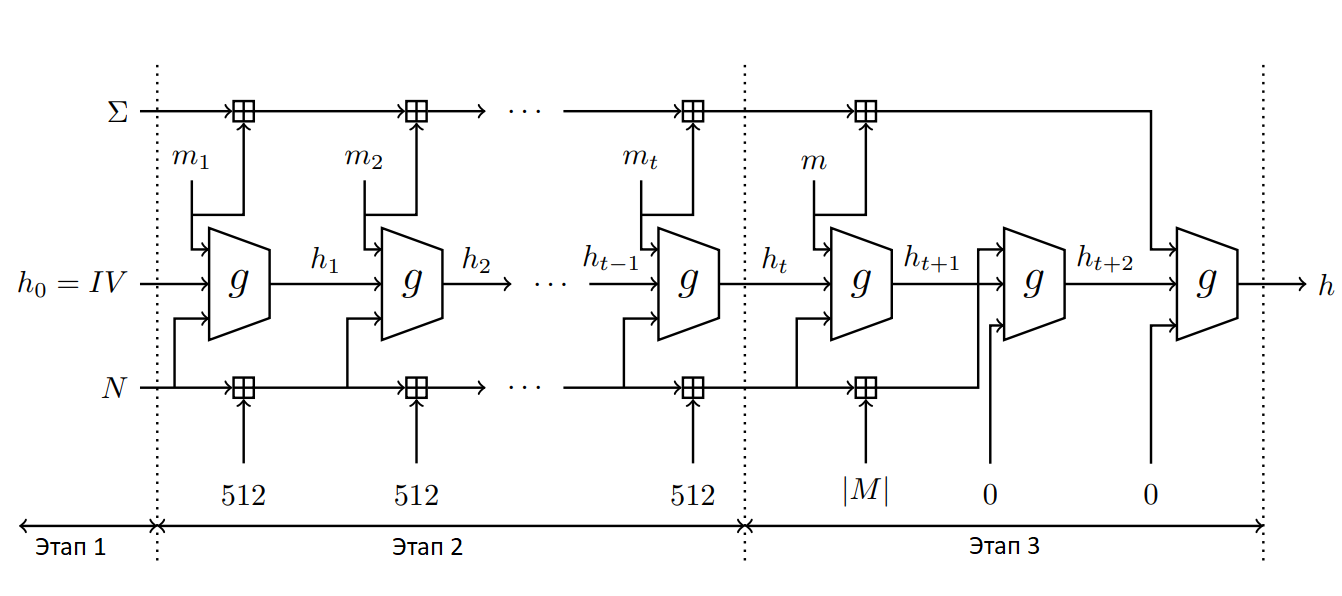
\includegraphics[width=1.0\linewidth]{inc/img/2_1}
		\caption{Схема вычисления хэш-функции. В случае длины хэша равной 256 бит возвращается $MSB_{256}(h)$.}
		\label{fig:fig2_1}
	\end{figure}
